\section{Installation}

\subsection{Binaries}
The easiest way to install ISSM is to download the
\href{https://issm.jpl.nasa.gov/download/binaries/}{pre-compiled binaries}. No need to compile the
code, just open the compressed file.

\subsection{Citations}
Inversions where first introduced to glaciology by \cite{MacAyeal1993a} for an SSA model, and extended since to 3D models for other model parameters.

Now, let's run our transient with historical mass balance! Use Jason Box's surface mass balance (SMB) time series as forcing \citep{Box2013a,Box2013b,Box2013c}.\textsuperscript{1}

\textsuperscript{1} \small{The year 1840-2012 Greenland near surface air temperature (T) and land ice SMB reconstruction after Box [2013] is calibrated to RACMO2 output \citep{Meijgaard2008,Ettema2009,Broeke2009,Angelen2011}. The calibration for T and SMB components is based on the 53 year overlap period 1960-2012. The calibration for snow accumulation rate is shorter because ice core data availability drops after 1999. Calibration is made using linear regression coefficients for 5 km grid cells that match the average of the reconstruction to RACMO2. The RACMO2 data are resampled and reprojected from the native 0.1 deg ($\sim$10 km) grid to a 5 km grid better resolving areas where sharp gradients occur, especially near the ice margin where mass fluxes are largest. Several refinements are made to the Box [2013] temperature (T) and SMB reconstruction. Multiple station records now contribute to the near surface air temperature for each given year, month and grid cell in the domain while in Box [2013], data from the single highest correlating station yielded the reconstructed value. The estimation of values is made for a domain that includes land, sea, and ice. Box [2013] reconstructed T over only ice. A physically-based meltwater retention scheme \citep{Pfeffer1990,Pfeffer1991} replaces the simpler approach used by Box [2013]. The RACMO2 data have a higher native resolution of 11 km as compared to the 24 km Polar MM5 data used by Box [2013] for air temperatures. The revised surface mass balance data end two years later in year 2012. The annual accumulation rates from ice cores are dispersed into a monthly temporal resolution by weighting the monthly fraction of the annual total for each grid cell in the domain evaluated using a 1960-2012 RACMO2 data.}

\subsubsection{Fonts}
\small{Small text} x\textsuperscript{2} H\textsubscript{2}O em dash-- Line break\\Some \emph{bold} text Some \it{italic} text
Here's a percentage sign: 100\%

\subsubsection{Equations}

\begin{equation}
	S(\theta,\phi,t) = \frac{R}{M} \left[ \mathcal{G}(\alpha) \otimes L(\theta',\phi',t) \right] +
	\frac{1}{g} \sum_{m=0}^{2} \sum_{i=1}^{2} \Lambda_{2mi} (t) \mathcal{Y}_{2mi} (\theta,\phi) +
	\mathcal{E}(t)
\end{equation}
\begin{equation}L(\theta,\phi,t) = \rho_I H(\theta,\phi,t) \mathcal{I}(\theta,\phi) + \rho_O S(\theta,\phi,t)
	\mathcal{O}(\theta,\phi)
\end{equation}
\begin{equation}
	S(\theta,\phi,t) = \frac{R}{M} \left[ \mathcal{G}(\alpha) \otimes L(\theta',\phi',t) \right] +
	\frac{1}{g} \sum_{m=0}^{2} \sum_{i=1}^{2} \Lambda_{2mi} (t) \mathcal{Y}_{2mi} (\theta,\phi) +
	\mathcal{E}(t)\end{equation}
\begin{equation}S(\theta,\phi,t) = \frac{R}{M} \left[ \mathcal{G}(\alpha) \otimes L(\theta',\phi',t) \right] + \frac{1}{g} \sum_{m=0}^{2} \sum_{i=1}^{2} \Lambda_{2mi} (t) \mathcal{Y}_{2mi} (\theta,\phi) + \mathcal{E}(t)\end{equation}

\subsubsection{Inline Equations}

where $y$ is a generic variable, $t$ indicates the model time step, $\overline{y}_{t}$ is the deterministic component of $y_{t}$, and $\epsilon_{y,t}$ is the stochastic perturbation applied at $t$ to $y$. The distribution of $\epsilon_{y}$ at any time step is Normal with a variance $\sigma^{2}_{y}$.

\begin{equation} \label{eq2}
    \boldsymbol{\epsilon}_{t} \sim N(\boldsymbol{0},\Sigma)
\end{equation}

where $\Sigma$ is the covariance matrix, and the bold font denotes vectors. If only the diagonal terms of $\Sigma$ are non-zero, all the individual entries of $\boldsymbol{\epsilon}_{t}$ are independent of each other. Covariance between the entries can be applied by adjusting the off-diagonal terms of $\Sigma$.

\subsubsection{vspace}

Some text followed by vspace
\vspace{3cm}
Some text following vspace


\subsubsection{Code folds}

Some text followed by a opening code fold %{{{
some text in the middle
closing code fold% }}}


\subsubsection{Figures}

Standard figure
\begin{figure}[H]
	\begin{center}
		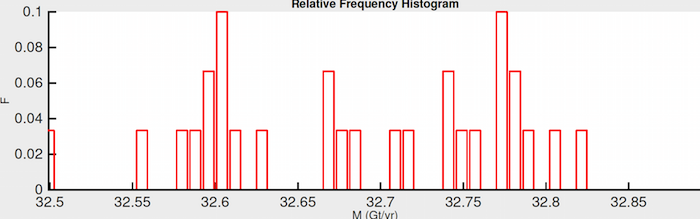
\includegraphics[scale=0.25]{../../../images/issm/documentation/tutorials/uncertaintyquantification/SamplingResults.png}
	\end{center}
\end{figure}

Figure containing two figures
\begin{figure}[H]
	\begin{center}
		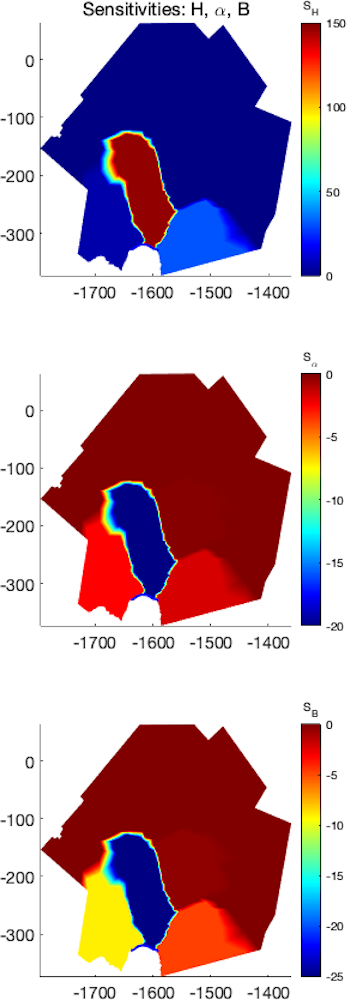
\includegraphics[scale=0.4]{../../../images/issm/documentation/tutorials/uncertaintyquantification/PlotSensitivities.png}
		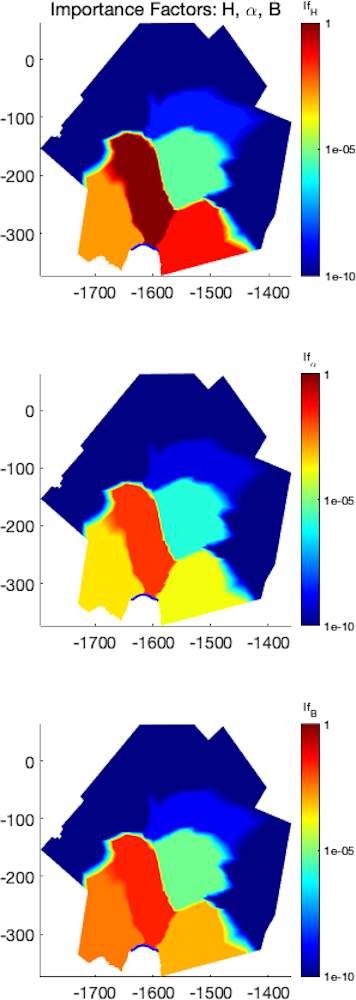
\includegraphics[scale=0.4]{../../../images/issm/documentation/tutorials/uncertaintyquantification/ImportanceFactors.png}
	\end{center}
\end{figure}

Figure with caption
\begin{figure}[H]
	\begin{center}
		\includegraphics{../../../images/issm/documentation/picop/picop.png}
		\caption{Melt calculation in PICOP, adapted from \cite{Pelle2019}.}
	\end{center}
\end{figure}

Another figure with a different caption
\begin{figure}[H]
	\begin{center}
		\caption{A great new caption}
		\includegraphics{../../../images/issm/documentation/picop/picop.png}
	\end{center}
\end{figure}


\subsubsection{Test nested substitutions}
Some text with \verb@%nested substitutions@ but here we have a literal percent % then \verb@another bit of verbatim text@ 

\subsubsection{.bashrc}
\begin{itemize}
	\item Open \verb@/c/msys64/home/<user>/.bashrc@ for editing and add the following at the bottom of the file, 
\begin{verbatim}## MATLAB
#
MATLAB_VER="<MATLAB_VER>" # Allows for easy resetting of MATLAB version added to path
export MATLAB_PATH=$(cygpath -u $(cygpath -ms "/c/Program Files/MATLAB/${MATLAB_VER}"))
export PATH="${MATLAB_PATH}/bin:${PATH}"

## ISSM
#
export ISSM_DIR=<ISSM_DIR>
export ISSM_DIR_WIN=$(cygpath -ms "${ISSM_DIR}") # Needed by MATLAB\end{verbatim}
where \verb@<MATLAB_VER>@ is the version of MATLAB that you have installed (for example, "R2023b")
and \verb@<ISSM_DIR>@ is the path to your local copy of the ISSM source code repository (for example, \verb@/c/Users/<USER>/ISSM@, where <USER> is your username)
	\item Another item
	\begin{itemize}
		\itemNested list item
		\item Another nested list item
	\end{itemize}
\end{itemize}
\begin{verbatim}
Another code block that follows a nested list
with different content but following text contains a new line\end{verbatim}
this is the following text preceded and followed by a new line
\subsection{Microsoft MPI}
\begin{itemize}
	\item Navigate to \url{https://docs.microsoft.com/en-us/message-passing-interface/microsoft-mpi-release-notes}
	\item Click the link for 'Microsoft Download Center' that corresponds with the latest release (take note of the version number that you download for the next step; it can also be found by going to 'Settings' / 'Apps & Features')
	\item Click the 'Download' button
	\begin{enumerate}
		\item Redistributions of source code must retain the above copyright notice,
		this list of conditions and the following disclaimer.
		\item Redistributions in binary form must reproduce the above copyright
			notice, this list of conditions and the following disclaimer in the
			documentation and/or other materials provided with the distribution.
		\begin{itemize}
			\item Ordered list item 1
			\item Ordered list item 2
			\item Ordered list item 3
		\end{itemize}
		\item Neither the name of the California Institute of Technology (Caltech),
			its operating division the Jet Propulsion Laboratory (JPL), the National
			Aeronautics and Space Administration (NASA), nor the names of its
			contributors may be used to endorse or promote products derived from
			this software without specific prior written permission.
	\end{enumerate}
	\item Make sure both boxes are checked, then click the 'Next' button
	\item Click the 'Save File' button for each file
	\item When the download completes, run each installer
	\item Follow the prompts, using the default installation directories
\end{itemize}
\subsection{Source Code}
If you would like to install ISSM from source, you will need to download the source code first. The
source code of ISSM is available on \href{https://github.com/ISSMteam/ISSM}{GitHub}. It can be
downloaded via https with,
\begin{verbatim}git clone https://github.com/ISSMteam/ISSM.git\end{verbatim}
or \verb@ssh@ with,
\begin{verbatim}git clone git@github.com:ISSMteam/ISSM.git\end{verbatim}
This will download the latest version of ISSM from the repository into the current local directory (or to the location of your choosing by passing a path as an optional argument to the command). 

If you downloaded the source code, you need to compile and install ISSM. Compilation of the ISSM
source code is theoretically possible on any platform. It has been successfully carried out on
Linux, macOS, and Windows. Here are some instructions to compile and install ISSM from the source
code:
%__@HTML_ONLY_START@__
%<!--DATASETS LIST START-->
%__@HTML_ONLY_END@__
\begin{itemize}
	\item A list item without any other markup
	\item \href{https://issm.jpl.nasa.gov/download/unix}{Linux/Mac}
	\item \href{https://issm.jpl.nasa.gov/download/windows}{Windows} (under development)
	\item A list item without any other markup
	\item \href{https://issm.jpl.nasa.gov/download/autodiff}{Installation with AD capability} (under development)
	\item \href{https://issm.jpl.nasa.gov/download/se}{Installation with Solid Earth capability} (under development)
	\item A list item without any other markup
\end{itemize}
%__@HTML_ONLY_START@__
%<!--DATASETS LIST END-->
%__@HTML_ONLY_END@__
Compilation is a more involved process, which is not recommended for beginners or casual users.

\subsection{License}
ISSM is released under a \href{https://opensource.org/license/bsd-3-clause}{BSD Three Clause License}.

Copyright (c) 2008-2024, California Institute of Technology.
All rights reserved. Based on Government Sponsored Research under contracts NAS7-1407 and/or NAS7-03001.

Redistribution and use in source and binary forms, with or without modification, are permitted provided that the following conditions are met:

\begin{enumerate}
	\item Redistributions of source code must retain the above copyright notice,
		this list of conditions and the following disclaimer.
	\item Redistributions in binary form must reproduce the above copyright
		notice, this list of conditions and the following disclaimer in the
		documentation and/or other materials provided with the distribution.
	\item Neither the name of the California Institute of Technology (Caltech),
		its operating division the Jet Propulsion Laboratory (JPL), the National
		Aeronautics and Space Administration (NASA), nor the names of its
		contributors may be used to endorse or promote products derived from
		this software without specific prior written permission.
\end{enumerate}

THIS SOFTWARE IS PROVIDED BY THE COPYRIGHT HOLDERS AND CONTRIBUTORS "AS IS" AND ANY EXPRESS OR IMPLIED WARRANTIES, INCLUDING, BUT NOT LIMITED TO, THE IMPLIED WARRANTIES OF MERCHANTABILITY AND FITNESS FOR A PARTICULAR PURPOSE ARE DISCLAIMED. IN NO EVENT SHALL THE CALIFORNIA INSTITUTE OF TECHNOLOGY BE LIABLE FOR ANY DIRECT, INDIRECT, INCIDENTAL, SPECIAL, EXEMPLARY, OR CONSEQUENTIAL DAMAGES (INCLUDING, BUT NOT LIMITED TO, PROCUREMENT OF SUBSTITUTE GOODS OR SERVICES; LOSS OF USE, DATA, OR PROFITS; OR BUSINESS INTERRUPTION) HOWEVER CAUSED AND ON ANY THEORY OF LIABILITY, WHETHER IN CONTRACT, STRICT LIABILITY, OR TORT (INCLUDING NEGLIGENCE OR OTHERWISE) ARISING IN ANY WAY OUT OF THE USE OF THIS SOFTWARE, EVEN IF ADVISED OF THE POSSIBILITY OF SUCH DAMAGE.
